\documentclass{article}
\usepackage{graphicx}
\usepackage[utf8]{inputenc}
\usepackage{amsmath, amssymb, latexsym}
 
\usepackage{pgfplots}
\usepackage{tikz}
\usepackage{nicefrac}
\pgfplotsset{every axis legend/.append style={
at={(0,0)},
anchor=north east}}
\usetikzlibrary{shapes,positioning,intersections,quotes}

\definecolor{darkgreen}{rgb}{0.0, 0.6, 0.0}
\definecolor{darkred}{rgb}{0.7, 0.0, 0.0}
\begin{document}


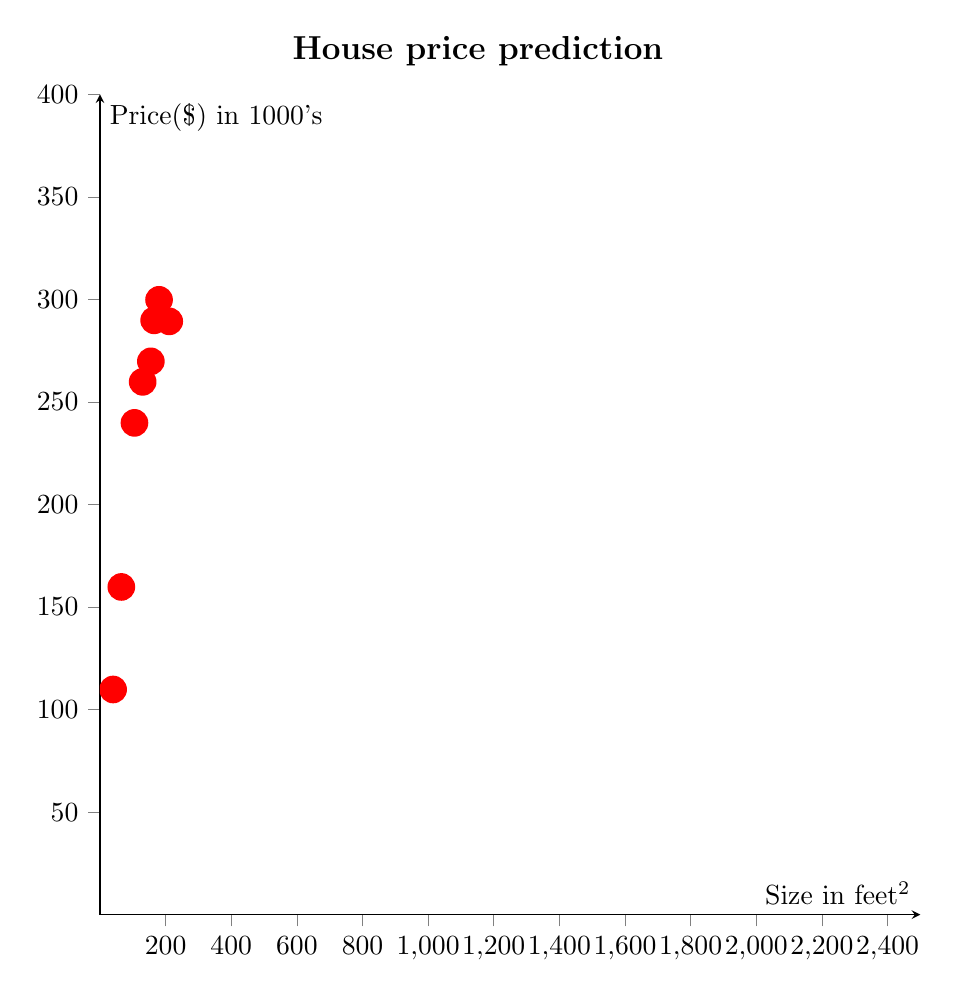
\begin{tikzpicture}
  \begin{axis}[
      axis x line=middle,
      axis y line=middle,
      width=12cm, height=12cm,     % size of the image
      grid = none,
      grid style={dashed, gray!0},
      %xmode=log,log basis x=10,
      %ymode=log,log basis y=10,
      xmin=0,     % start the diagram at this x-coordinate
      xmax= 2500,    % end   the diagram at this x-coordinate
      ymin=0,     % start the diagram at this y-coordinate
      ymax= 400,   % end   the diagram at this y-coordinate
      %/pgfplots/xtick={0,1,...,60}, % make steps of length 5
      %extra x ticks={23},
      %extra y ticks={0.507297},
      axis background/.style={fill=white},
      ylabel=Price(\$) in 1000's,
      xlabel=Size in feet$^2$,
      %xticklabels={,,},
      %yticklabels={,,},
      tick align=outside,
      tension=0.08]
    % plot the stirling-formulae
    \fill[red] (211, 289.3) circle (5pt);
    \fill[red] (180, 299.8) circle (5pt);
    \fill[red] (165, 289.8) circle (5pt);
    \fill[red] (130, 259.8) circle (5pt);
    \fill[red] (155, 269.8) circle (5pt);
    \fill[red] (105, 239.8) circle (5pt);
    \fill[red] (65, 159.8) circle (5pt);
    \fill[red] (40, 109.8) circle (5pt);
  \end{axis}
  \node[above,font=\large\bfseries] at (current bounding box.north) {House price prediction};
\end{tikzpicture}

\end{document}